\documentclass{theme/uniprthesis}

%%%%%%%%%%%Some Extra Packages%%%%%%%%%%%
\usepackage[italian]{babel}		% To have Italina names in Sections, Figures, Chapters etc.
\usepackage{todonotes}			% To ease the revision


\usepackage{blindtext} 			% Dummy Text - remove
%%%%%%%%%%%%%%%%%%%%%%%%%%%%%%%%%


%%%%% THESIS / TITLE PAGE INFORMATION
% Everybody needs to complete the following:

\title{Titolo in Italiano}
\author{Saverio Mattia Merenda}
\advisor{Prof. Vincenzo Arceri}
\college{Dipartimento di Scienze Matematiche, Fisiche e Informatiche}
\degree{Corso di Laurea Triennale in Informatica}
\degreeyears{2023--2024}


% Not mandatory fields
% \newcommand{\subTitle}{Titolo in Inglese} %Subtitle, usually the english version of the title

%\newcommand{\advisorSecond}{Prof. Nome2 Cognome2} % For multiple (up to 4) advisors -- if this is not present then also the remaining ones are automatically omitted
%\newcommand{\advisorThird}{Dott. Nome3 Cognome3} % For multiple (up to 4) advisors -- if this is not present then also the remaining ones are automatically omitted
%\newcommand{\advisorFourth}{Dott. Nome4 Cognome4} % For multiple (up to 4) advisors

%\newcommand{\coadvisor}{Prof. co-Nome co-Cognome} %For multiple (up to 4) coadvisors -- if this is not present then also the remaining ones are automatically omitted
%\newcommand{\coadvisorSecond}{Prof. co-Nome2 co-Cognome2} % For multiple (up to 4) coadvisors -- if this is not present then also the remaining ones are automatically omitted
%\newcommand{\coadvisorThird}{Dott. co-Nome3 co-Cognome3} % For multiple (up to 4) coadvisors -- if this is not present then also the remaining ones are automatically omitted
%\newcommand{\coadvisorFourth}{Dott. co-Nome4 co-Cognome4} % For multiple (up to 4) coadvisors


\begin{document}

\maketitle

%%%% La dedica
\newpage
\thispagestyle{empty}
\null\vspace{\stretch{1}}
\begin{flushright}
	\textit{A me medesimo.}
\end{flushright}
\vspace{\stretch{3}}\null
\newpage

%%%% Gli indici
\pagestyle{plain}
\pagenumbering{roman}
\tableofcontents

\listoffigures    %Commentare se non vi sono Immagini
\listofalgorithms %Commentare se non vi sono Algoritmi
%\listoftables     %Commentare se non vi sono Tabelle

%%%% La prefazione
\chapter*{Introduzione} 
\addcontentsline{toc}{chapter}{Introduzione} 
\pagenumbering{arabic} 
Ethereum \cite{wood2014ethereum} è una piattaforma blockchain che consente la creazione di un ambiente globale decentralizzato, 
in cui gli utenti possono sviluppare strumenti digitali sicuri utilizzando la valuta nativa Ether (ETH) per transazioni e servizi 
computazionali.

La rete Ethereum è costituita da nodi interconnessi che seguono regole definite nel protocollo Ethereum, supportando una vasta 
gamma di comunità, applicazioni, organizzazioni e attività digitali accessibili a chiunque abbia una connessione internet.

La caratteristica principale di Ethereum è la capacità di eseguire smart contract tramite la Ethereum Virtual Machine (EVM), 
consentendo funzionalità avanzate al di là delle transazioni finanziarie di base (e.g. Bitcoin \cite{nakamoto2008bitcoin}). 
Gli smart contract sono programmi immutabili memorizzati sulla blockchain che eseguono azioni predefinite senza intervento umano.

Tuttavia, garantire la sicurezza e l’affidabilità degli smart contract è essenziale, poiché non possono essere modificati una 
volta deployati. La presenza di bug o vulnerabilità potrebbe causare gravi conseguenze, come perdite di fondi o azioni indesiderate.

Per garantire la qualità degli smart contract, vengono sviluppate tecniche di analisi e verifica del codice. L’analisi statica, 
ad esempio, identifica potenziali problemi di sicurezza senza eseguire effettivamente il codice. Tuttavia, nel contesto di Ethereum, 
la costruzione di un Control Flow Graph (CFG) affidabile è complessa a causa delle destinazioni dinamiche dei salti (Jump Orfane) 
durante l’esecuzione del EVM bytecode.

In questo elaborato viene presentato EVMLiSA \footnote{\url{https://github.com/lisa-analyzer/evm-lisa}.}, un software in grado di 
costruire un CFG sound e affidabile (TODO si spera) di smart contract eseguibili su EVM.

%%%% I capitoli di Contenuto	
\pagestyle{fancy}
% \include{capitoli/Formattazione}
\chapter{Background}\label{chapter:background}
TODO scrivere riassuntino

\section{Blockchain}\label{sec:blockchain}
Il concetto di blockchain è stato introdotto per la prima volta nel 2008 da Satoshi Nakamoto con il whitepaper 
di Bitcoin \cite{nakamoto2008bitcoin} e successivamente implementato nel 2009 come tecnologia alla base di Bitcoin.

È importante sottolineare che Bitcoin e blockchain sono due entità separate: Bitcoin rappresenta solo una delle 
molteplici applicazioni costruite sulla tecnologia blockchain.

La blockchain è un registro digitale, decentralizzato e distribuito su una rete, strutturato come una catena di 
blocchi responsabili dell’archiviazione dei dati. Questi dati possono comprendere informazioni di valore economico 
o intere applicazioni digitali. È possibile aggiungere nuovi blocchi di informazioni, ma non è possibile modificare 
o rimuovere i blocchi precedentemente aggiunti alla catena.

In questo ambiente, la crittografia e i protocolli di consenso garantiscono sicurezza e immutabilità. Il risultato 
è un sistema aperto, neutrale, affidabile e sicuro, dove la nostra capacità di utilizzare e fidarci del sistema non 
dipende dalle intenzioni di nessun individuo o istituzione.

La blockchain può essere considerata parte della famiglia delle Distributed Ledger Technology (DLT): tutti i 
partecipanti alla rete hanno accesso al registro distribuito e al suo registro immutabile delle transazioni. Questo 
registro condiviso consente di registrare le transazioni una sola volta, eliminando la duplicazione degli sforzi 
tipica delle reti aziendali tradizionali \cite{chiap2019blockchain}. 

\subsection{Funzionamento}\label{subsec:funzionamento}
La blockchain è composta da una serie di blocchi, aggiunti uno dopo l’altro in modo sequenziale. Ogni blocco contiene 
una prova matematica, resa possibile dall’utilizzo della crittografia, che ne assicura la sequenzialità tramite un 
hash del blocco precedente.

Sebbene il concetto di catena di blocchi sia comune a quasi tutti i sistemi blockchain, la struttura e il contenuto 
dei blocchi possono variare a seconda dello scopo della blockchain stessa. Ad esempio, i blocchi della blockchain di 
Bitcoin possono essere diversi da quelli della blockchain di Ethereum.

I blocchi sono interconnessi tramite funzioni di hash crittografiche (e.g. SHA-256 [TODO forse andrebbe spiegato?]), 
creando un legame matematico tra di loro. Questo processo fornisce un modo conveniente per esprimere l’intero contenuto 
della blockchain in una singola stringa di lunghezza definita.

Ogni blocco contiene informazioni specifiche (e.g. le transazioni) e l’hash del blocco precedente (Figura~\ref{fig:one}). 
Modificare qualsiasi informazione in un blocco altererebbe l’hash del blocco e, di conseguenza, tutti gli hash successivi, 
rendendo immediatamente evidente l’alterazione.

Ogni nuovo blocco rafforza la verifica dei blocchi precedenti, rendendo la blockchain a prova di manomissione e fornendo 
un registro affidabile delle transazioni su cui gli utenti possono fare affidamento \cite{chiap2019blockchain}. 

\begin{figure}[ht]
	\centering
	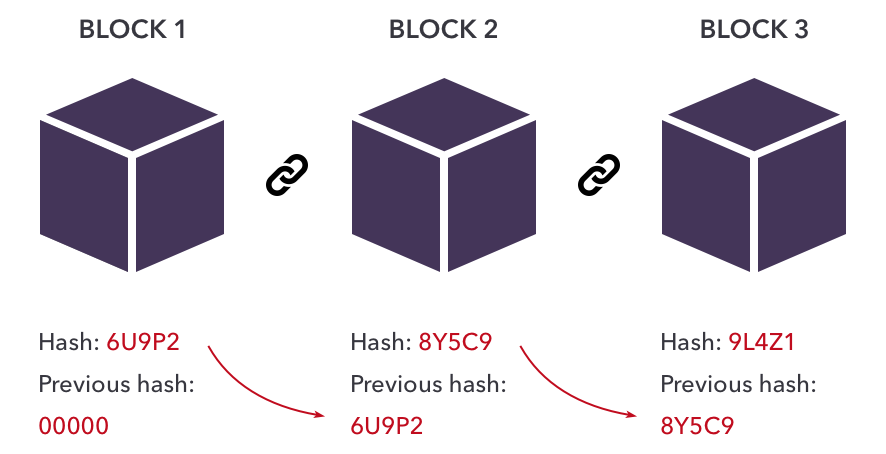
\includegraphics[width=0.8\textwidth]{Immagini/blockchain.png}
	\caption{Funzionamento della blockchain.}
	\label{fig:one}
\end{figure}

\subsection{Consenso}\label{subsec:consenso}
Il consenso è il processo mediante il quale i nodi della rete raggiungono un accordo su ciò che è avvenuto all’interno 
della blockchain. Questo accordo rappresenta l’unica verità sullo stato attuale della blockchain e viene ottenuto 
attraverso un accordo generale tra i partecipanti della rete. Il consenso non è un evento istantaneo, ma un processo 
continuo che coinvolge vari partecipanti con ruoli e responsabilità specifici. Si basa su principi matematici ed e
conomici per incentivare tutti i membri a raggiungere un accordo su un unico dato \cite{chiap2019blockchain}. 

Nella pratica, il consenso richiede che i nuovi blocchi siano approvati dalla maggioranza dei nodi della rete, che 
sono distribuiti su una vasta rete di computer. Questo processo può avvenire attraverso due meccanismi principali: 
la Proof of Work (PoW) e la Proof of Stake (PoS).

\begin{itemize}
    \item Proof of Work (PoW): È il sistema di consenso utilizzato principalmente da Bitcoin. Qui, i nodi della rete, 
        noti come “miner”, competono per risolvere complessi problemi crittografici. Il primo nodo che risolve con 
        successo il problema crittografico viene premiato con una quantità specifica di criptovaluta. La difficoltà 
        di generare l’hash viene modificata man mano che la rete si espande, in modo che i nuovi blocchi vengano creati 
        e approvati a un ritmo costante al variare della potenza di calcolo della rete. La difficoltà di generare blocchi 
        nella blockchain di Bitcoin, ad esempio, viene regolata modificando il numero di zeri con cui devono iniziare, 
        garantendo che un nuovo hash venga trovato solo una volta ogni dieci minuti circa dall’intera rete. Questi problemi 
        sono progettati per richiedere una grande quantità di potenza di calcolo e l’energia utilizzata in questo processo 
        è sia una caratteristica distintiva che un punto di vulnerabilità di PoW. Se da un lato rende la blockchain sicura, 
        poiché sarebbe estremamente costoso e poco pratico per un singolo attaccante possedere la maggior parte della potenza 
        di calcolo della rete, dall’altro richiede una notevole quantità di energia elettrica \cite{davidetarpini}.
    
    \item Proof of Stake (PoS): È un meccanismo di consenso in cui i nodi della rete, chiamati “validatori”, competono per 
        essere selezionati per convalidare il prossimo blocco. La probabilità di essere selezionati è proporzionale alla 
        quantità di criptovaluta che il nodo ha depositato nella blockchain. Quando un validatore viene selezionato, 
        “mette in gioco” (stake) i propri fondi (token). Se il validatore non adempie ai propri doveri o tenta di commettere 
        una frode, rischia di perdere i suoi fondi. PoS non richiede una quantità significativa di energia elettrica come PoW, 
        ma presenta un problema di monopolio della ricchezza, poiché coloro che possiedono più token hanno maggiori 
        probabilità di essere selezionati per convalidare il blocco successivo e ricevere la ricompensa. Questo problema è 
        mitigato con l’introduzione di Delegated Proof of Stake (DPoS), che prevede un sistema di voto per la selezione dei 
        validatori, rendendo il processo più democratico \cite{davidetarpini}.
\end{itemize}

\subsection{Classificazione delle blockchain}\label{subsec:classificazione}
Le blockchain possono essere categorizzate in vari tipi in base alla loro accessibilità e ai requisiti di utilizzo:

\begin{itemize}
    \item Permissionless: Questo tipo di blockchain permette a chiunque di accedervi senza restrizioni, senza la necessità di 
        identificarsi. Esempi notevoli sono Bitcoin ed Ethereum. Tuttavia, questa libertà può portare a problemi di dimensionamento 
        e sicurezza, poiché ogni nodo della rete deve elaborare e convalidare l’intera blockchain, rendendo anche più probabile 
        l’ingresso di attori malevoli \cite{permission}.

    \item Permissioned: Al contrario, nelle blockchain ad accesso limitato, l’accesso è controllato e richiede l’autenticazione 
        da parte di un’autorità centrale. Questo approccio riduce i problemi di dimensionamento e sicurezza riscontrati nelle 
        blockchain aperte. Tuttavia, l’intervento di un’autorità centrale compromette parzialmente il principio di decentralizzazione
        \cite{permission}.
\end{itemize}

Ulteriormente, le blockchain possono essere suddivise in base alle loro applicazioni e requisiti specifici:

\begin{itemize}
    \item Public: Le blockchain pubbliche incoraggiano la partecipazione di tutti gli utenti, offrendo incentivi come ricompense 
        in criptovaluta. Sono trasparenti e flessibili. Esempi ben noti includono Bitcoin ed Ethereum \cite{toshendra}.

    \item Private: Le blockchain private sono utilizzate all’interno di reti aziendali o organizzative, spesso per migliorare 
        l’efficienza dei processi interni. Sono meno trasparenti rispetto alle blockchain pubbliche e richiedono solitamente 
        un’autorizzazione per accedervi \cite{toshendra}.

    \item Consortium: Queste blockchain sono progettate per la collaborazione tra più entità, come aziende o istituzioni. La 
        gestione dell’accesso è condivisa tra i partecipanti, garantendo un certo livello di decentralizzazione senza dipendenza 
        da un’autorità centrale \cite{toshendra}.
\end{itemize}

\subsection{Chiave pubblica e chiave privata}\label{subsec:chiavi}
TODO non so se metterlo o no

%%%%%%%%%%%%%%%%%%%%%%%%%%%%%%%%%%%%%%%%%%%%%%%%%%%%%%%%%%%%%%%%%%%%%%%%%%%%%%%%%%%%%%%%

\newpage
\section{Ethereum}\label{sec:ethereum}
Ethereum è una blockchain aperta (permissionless), accessibile a chiunque (pubblica) e con il codice sorgente disponibile 
liberamente (open-source). È stata ideata per la prima volta da Vitalik Buterin nel 2013 \cite{buterin2013ethereum}, con 
l’obiettivo di creare una blockchain in grado di eseguire una vasta gamma di programmi generici.

Dal punto di vista tecnico, Ethereum può essere considerato una sorta di enorme macchina virtuale globale e “infinita”, 
che opera seguendo uno stato singolo accessibile da qualsiasi parte del mondo e una macchina virtuale che applica le 
modifiche a tale stato.

Tuttavia, in termini più pratici, Ethereum si presenta come un’infrastruttura informatica decentralizzata, aperta a tutti 
e basata su codice sorgente accessibile \footnote{\url{https://github.com/ethereum/go-ethereum}}, che consente l’esecuzione 
di programmi denominati Smart Contracts (Sezione \ref*{sec:smartContracts}). Utilizza una blockchain per tenere traccia e 
registrare le variazioni di stato del sistema, utilizzando la criptovaluta nativa (chiamata Ether) per misurare e regolare 
i costi delle risorse di elaborazione.

Attraverso la piattaforma Ethereum, gli sviluppatori hanno la possibilità di creare applicazioni decentralizzate con funzioni 
economiche integrate, offrendo non solo elevata disponibilità, verificabilità, trasparenza e neutralità, ma anche la riduzione 
o l’eliminazione della censura e alcuni rischi associati alle controparti tradizionali \cite{antonopoulos2018mastering}.

\subsection{Etherem vs Bitcoin}\label{subsec:ethVSbtc}
Ethereum presenta numerose caratteristiche comuni con altre blockchain aperte: una rete peer-to-peer che collega gli utenti, 
un algoritmo di consenso per mantenere gli aggiornamenti di stato sincronizzati (inizialmente basato su un consenso proof-of-work, 
ma con l’avvento dell’aggiornamento “The Merge” \footnote{\url{https://ethereum.org/it/roadmap/merge/}}, il consenso è passato 
a proof-of-stake), l’uso di tecniche crittografiche come firme digitali e hash, e una valuta digitale (ETH).

Tuttavia, sia lo scopo che la struttura di Ethereum si differenziano notevolmente da quelle delle blockchain precedenti, come Bitcoin.

Il principale obiettivo di Ethereum non è solo quello di fungere da sistema di pagamento digitale. Anche se l’ether è fondamentale 
per il funzionamento di Ethereum, essa viene considerata una “valuta di utilità” utilizzata per pagare l’utilizzo della piattaforma 
Ethereum come un computer globale.

A differenza di Bitcoin, che dispone di un linguaggio di scripting limitato, Ethereum è stato progettato per essere una blockchain 
programmabile per scopi generici, con una macchina virtuale EVM in grado di eseguire codice di complessità arbitraria e illimitata. 
Mentre il linguaggio di scripting di Bitcoin si limita principalmente a valutazioni semplici (true/false) delle condizioni di spesa 
di un utente, il linguaggio di Ethereum (Solidity \footnote{\url{https://docs.soliditylang.org/en/latest/}}) è quasi completo in 
termini di capacità computazionale (Turing completeness), consentendo ad Ethereum di funzionare come un computer per scopi 
generali \cite{antonopoulos2018mastering}.

\subsection{Funzionamento}\label{subsec:funzionamentoETH}
Sulla blockchain Ethereum sistono due tipi principali di account utilizzabili per gestire le transazioni e l’interazione sulla rete: 
gli Externally Owned Account e i Contract Account.

Gli Externally Owned Account (EOA) sono controllati direttamente dagli utenti e sono associati a una coppia di chiavi crittografiche, 
pubblica e privata. Questi account consentono agli individui di ricevere e inviare ether e di partecipare alle transazioni sulla rete. 
Le transazioni tra due account esterni coinvolgono esclusivamente lo scambio di ether e non comportano alcun costo di creazione 
dell’account \cite{ethereumaccounts}.

I Contract Account, invece, sono associati agli smart contract. Questi account contengono il codice dello smart contract e vengono 
attivati quando ricevono una transazione. Le transazioni con questi account possono coinvolgere l’esecuzione di codice dello smart 
contract, oltre allo scambio di ether e comportano un costo di creazione in quanto richiedono risorse di calcolo e di archiviazione 
sulla rete Ethereum \cite{ethereumaccounts}.

Affinché una transazione venga effettuata su Ethereum, il mittente deve conoscere l’indirizzo del destinatario, detto anche chiave 
pubblica dell’account, e firmare digitalmente la transazione con la propria chiave privata. Questo processo dimostra che il richiedente 
della transazione è il legittimo proprietario dell’account.

Le transazioni sono essenzialmente istruzioni crittograficamente firmate da un account che iniziano una modifica dello stato della 
rete Ethereum. Inoltre, per “transazione” si intende una transazione approvata e inclusa in un blocco della blockchain.

Poiché le transazioni sono atomiche, esse devono essere eseguite completamente prima di apportare cambiamenti allo stato globale della 
rete. Questo significa che tutte le istruzioni all’interno della transazione devono essere valide. Se una qualsiasi istruzione fallisce, 
gli effetti della transazione vengono annullati e lo stato viene ripristinato al momento precedente (rollback), come se la transazione 
non fosse mai avvenuta. Anche se una transazione fallisce, viene comunque registrata come tentata, ma non influenza lo stato complessivo 
della rete \cite{ethereumsmartcontracts}.

Ogni transazione su Ethereum comporta un costo proporzionale alla sua complessità computazionale, misurato in “gas”. Possiamo pensare al 
gas come al carburante necessario per far funzionare le operazioni sulla blockchain, simile al carburante utilizzato da un’auto per 
percorrere una determinata distanza.

Ogni operazione sulla blockchain ha un costo specifico in gas. Ad esempio, calcolare un hash o fare una somma di due numeri richiede una 
differente quantità di gas (30 e 3, rispettivamente). 

Il gas è misurato in “wei” ($1 \text{ wei } = 1^{-18} \text{ ETH }$) ed è strettamente legato alle transazioni. 
Ogni transazione su Ethereum ha due parametri: il prezzo del gas (gas price) e il limite del gas (gas limit), che rappresentano 
rispettivamente il prezzo che si è disposti a pagare per unità di gas e la quantità massima di gas utilizzabile.

A differenza di Bitcoin, dove esiste un limite alla dimensione massima di un blocco, su Ethereum si fa riferimento al limite di gas, che 
determina la massima quantità di calcoli che la Ethereum Virtual Machine deve eseguire per blocco.

Immaginiamo di dover eseguire una transazione che richiede 10 gas e abbiamo deciso di pagare 100 wei per ogni gas: il costo totale della 
transazione sarà di 1000 wei ($10 \times 100$). Se aumentiamo il prezzo del gas a 1000 wei per gas, il costo totale della transazione sarà di 
10000 wei ($10 \times 1000$). I validatori della rete Ethereum sono liberi di scegliere le transazioni da includere nel nuovo blocco, e 
generalmente cercano di massimizzare il profitto. Di conseguenza, le transazioni con un prezzo del gas più elevato hanno una priorità 
maggiore di essere aggiunte al blocco successivo.

Se una transazione richiede 15 gas ma abbiamo impostato un limite di 10 gas, l’esecuzione si interromperà quando verrà raggiunto il limite, 
e tutto il gas andrà perso. Se, invece, il limite di gas è superiore a quello utilizzato dalla transazione, il gas in eccesso verrà restituito 
al mittente.

Quindi, il costo totale di una transazione può essere calcolato con la seguente formula: 
$$\text{Costo transazione } = \text{ Limite di gas } \times \text{ Prezzo del gas}$$

Oltre a compensare i validatori, il costo delle transazioni su Ethereum serve anche a proteggere la blockchain da attacchi, come il DDoS, 
e da errori di programmazione negli smart contract che potrebbero sovraccaricare il sistema. Ad esempio, se una computazione finisse in 
un ciclo infinito, la gestione del gas interromperebbe l’esecuzione una volta che il gas disponibile è esaurito. Questa caratteristica 
ci consente di definire Ethereum come un linguaggio (quasi) Turing-completo, poiché siamo sicuri che ogni programma in esecuzione terminerà 
\cite{chiap2019blockchain}.

%%%%%%%%%%%%%%%%%%%%%%%%%%%%%%%%%%%%%%%%%%%%%%%%%%%%%%%%%%%%%%%%%%%%%%%%%%%%%%%%%%%%%%%%

\newpage
\section{Smart Contracts}\label{sec:smartContracts}
Il concetto di smart contract è stato introdotto per la prima volta da Nick Szabo nel 1996, definendolo come “un protocollo di transazione 
digitale che esegue i termini di un contratto” \cite{szabo1996smart}. Lo scopo principale di uno smart contract è quello di automatizzare 
l’adempimento delle condizioni contrattuali, riducendo al minimo il rischio di azioni malevole e la necessità di fidarsi degli intermediari 
(rischio di controparte).

Un contratto, in generale, è un accordo legalmente vincolante tra due o più parti e svolge un ruolo fondamentale nell’instaurare fiducia 
tra i soggetti coinvolti in una transazione \footnote{\url{https://www.treccani.it/enciclopedia/contratto/}}. Può essere tanto semplice 
quanto un biglietto dell’autobus o molto complesso come un contratto di lavoro.

Nel contesto delle blockchain, uno smart contract è un programma che replica tutte le caratteristiche di un contratto tradizionale, ma viene 
memorizzato ed eseguito all’interno di una blockchain. Si tratta di un agente autonomo che risiede su una blockchain, senza la necessità 
di un’entità esterna per valutare le condizioni e prendere decisioni. Questo ruolo è sostituito dal consenso della rete. Gli smart contract 
stabiliscono le regole e le fanno rispettare automaticamente alle parti coinvolte, senza la necessità di autorità centrali. Quando le 
condizioni del contratto vengono soddisfatte, lo smart contract esegue autonomamente azioni specifiche, come ad esempio il trasferimento 
di denaro \cite{chiap2019blockchain}.

Un smart contract può essere paragonato a un’applicazione IFTTT (If This Then That) che risponde a eventi specifici (Figura~\ref{fig:two}).

\begin{figure}[ht]
	\centering
	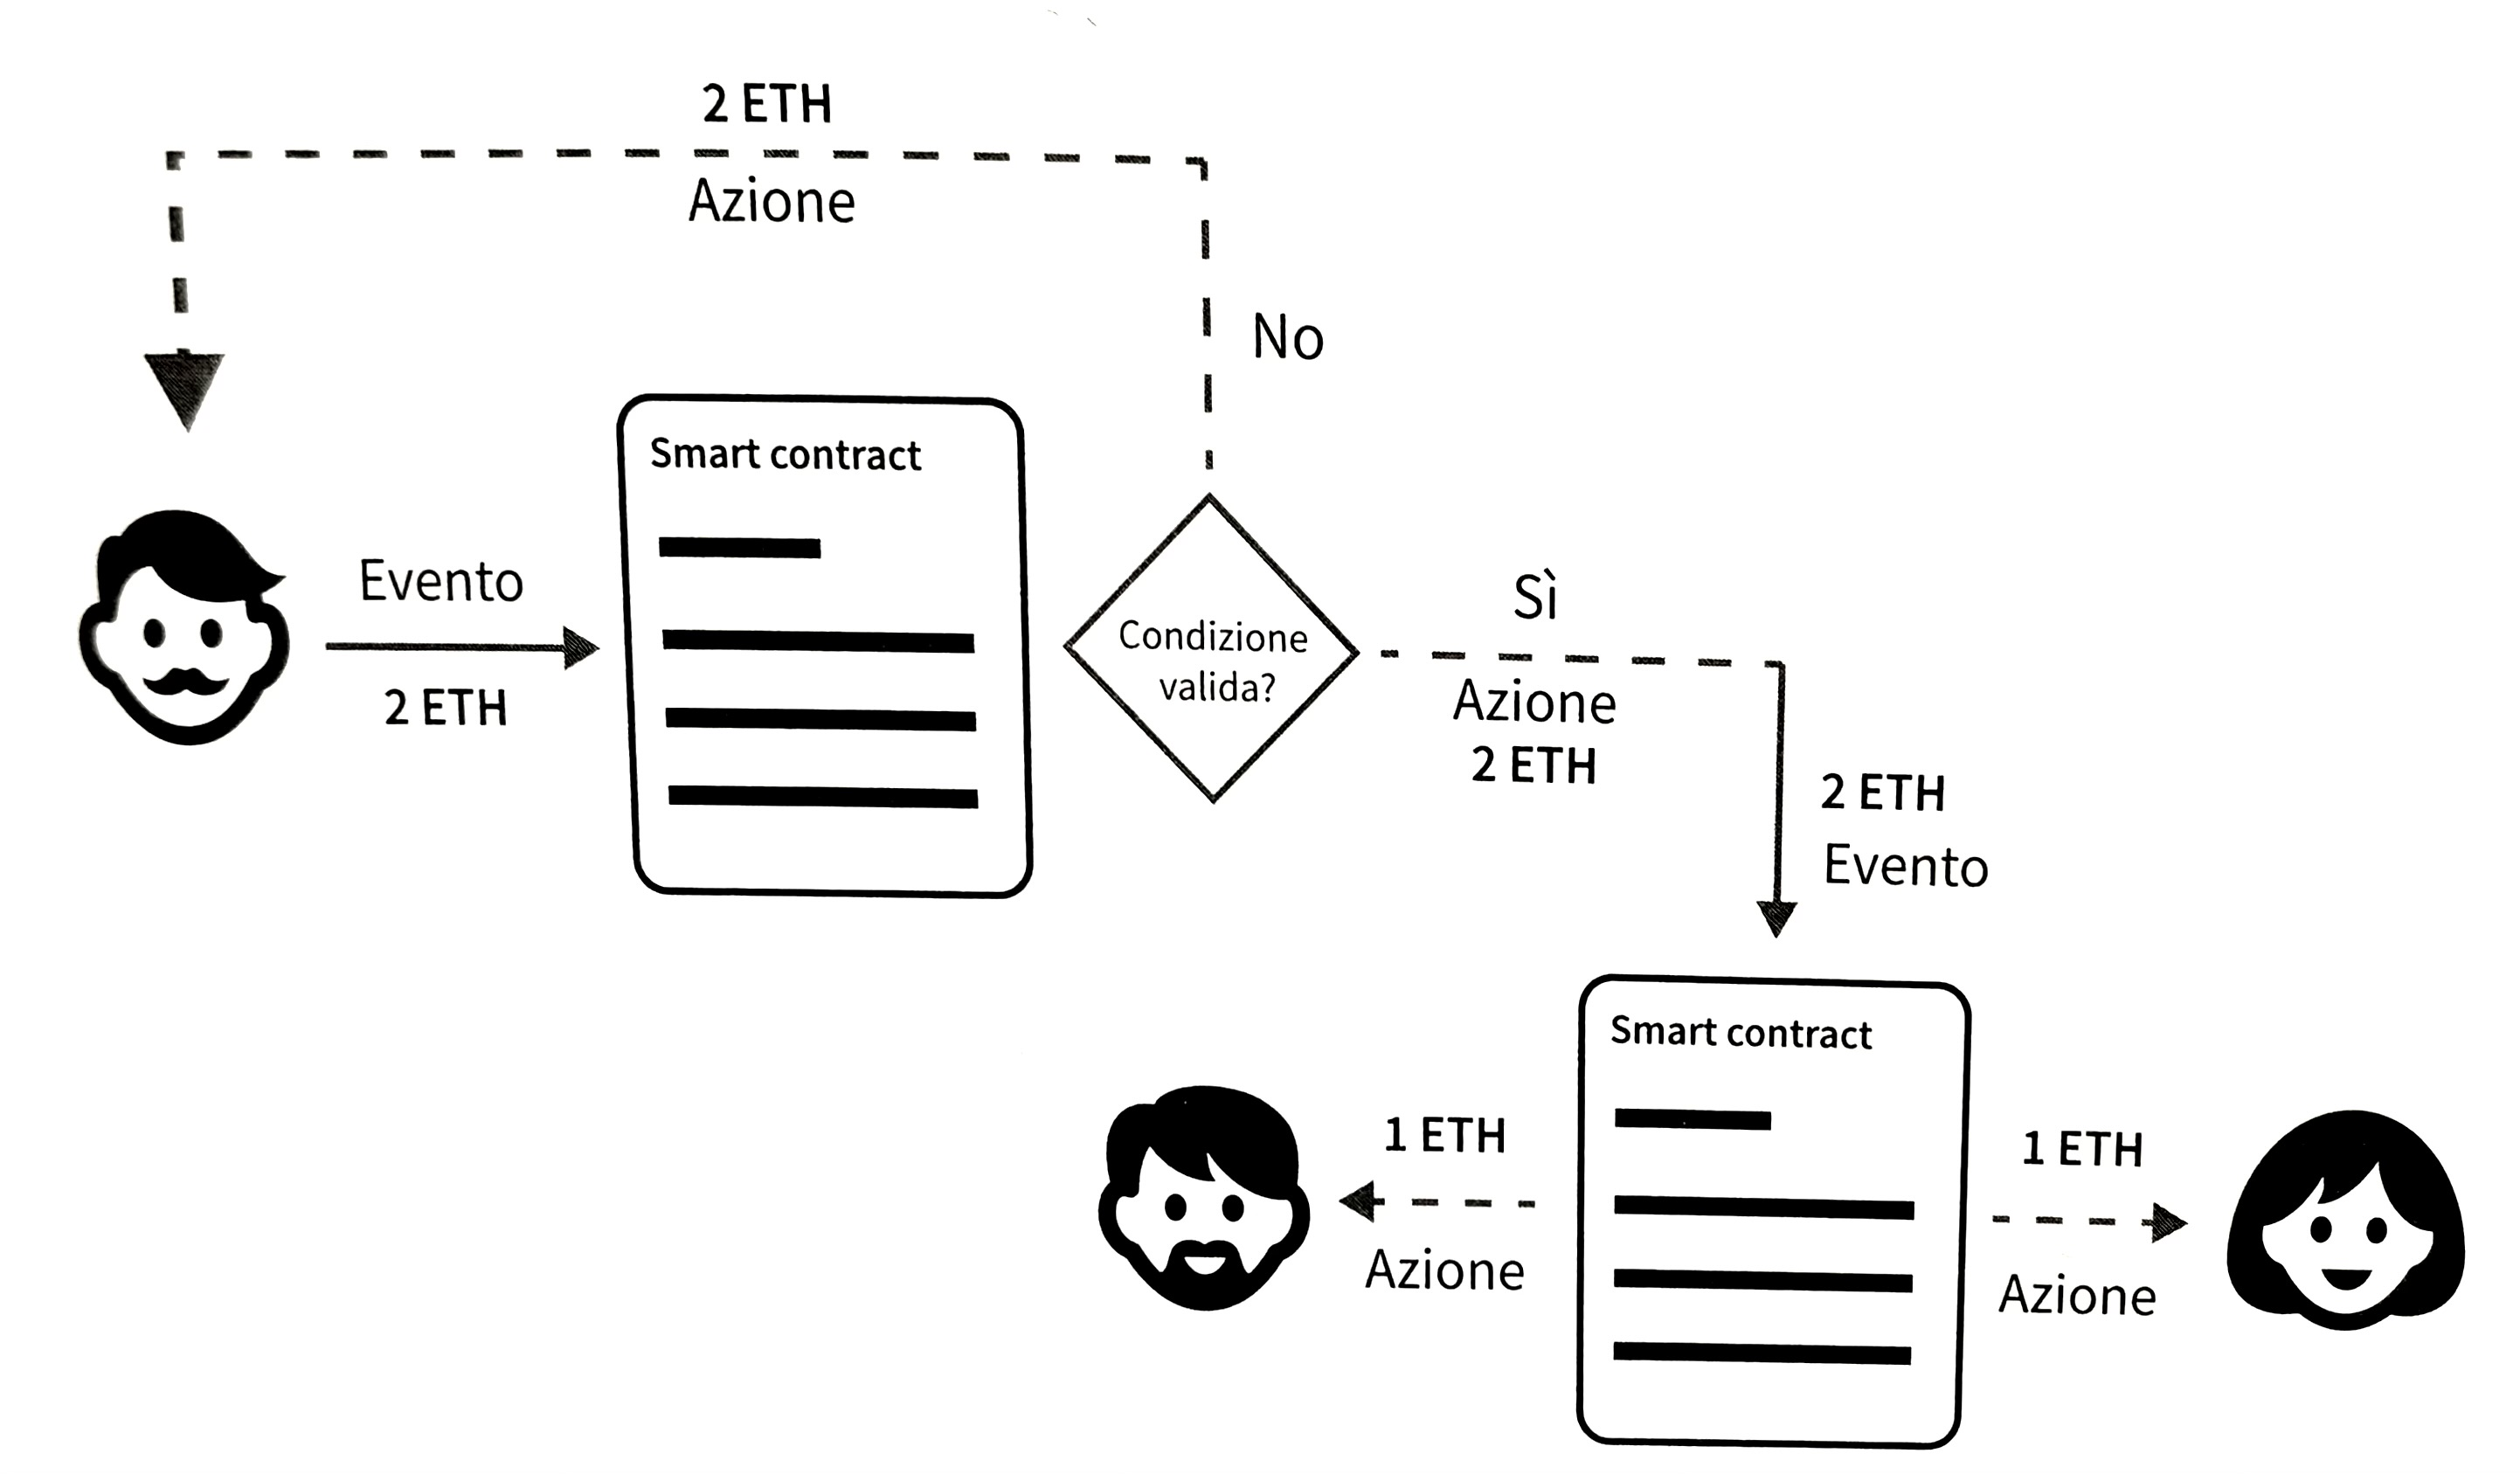
\includegraphics[width=0.8\textwidth]{Immagini/smart-contract.jpeg}
	\caption{Il processo IFTTT negli smart contracts \\ TODO sistemare con photoshop questa figura}
	\label{fig:two}
\end{figure}

Gli smart contract, solitamente redatti in un linguaggio di alto livello come Solidity, necessitano di essere compilati nel bytecode di basso 
livello eseguito nell’EVM per poter essere eseguiti. Dopo la compilazione, vengono distribuiti sulla piattaforma Ethereum attraverso una speciale 
transazione di creazione del contratto, inviata all’indirizzo di creazione del contratto {\tt 0x0}, detto \textit{zero address}. Ogni contratto è identificato 
da un indirizzo Ethereum, derivato dalla transazione di creazione del contratto in funzione dell’account di origine e del nonce. Come già 
menzionato nella sezione \ref*{subsec:funzionamentoETH}, a differenza degli EOAs, gli account creati per nuovi smart contract non hanno chiavi associate.

Gli smart contract vengono eseguiti solo quando vengono richiamati da una transazione. Ogni smart contract in Ethereum viene eseguito a seguito 
di una transazione avviata da un EOA. Un contratto può richiamare un altro contratto, che a sua volta può richiamare un altro contratto e così 
via, ma il primo contratto in questa catena di esecuzione sarà sempre stato richiamato da una transazione proveniente da un EOA.

Le transazioni sono atomiche, indipendentemente dal numero di smart contract richiamati o dalle azioni che eseguono. Ogni transazione viene 
eseguita nella sua totalità e le eventuali modifiche allo stato globale vengono registrate solo se l’esecuzione termina con successo. Se 
l’esecuzione fallisce a causa di un errore, tutti gli effetti vengono annullati e la transazione viene registrata come tentata.

È importante notare che una volta distribuito, il codice di un contratto non può essere modificato. Approfondiremo ulteriormente questo 
aspetto in seguito.

\subsection{Esempio di smart contract}\label{subsec:esempioSmartContract}
Ma adesso vediamo un esempio di smart contract 
\footnote{Tratto da: \url{https://solidity-by-example.org/sending-ether/}} 
nell' Algoritmo \ref*{lst:esempioSolidity}.

Questo smart contract è composto da due contratti: \textit{ReceiveEther} e \textit{SendEther}.

Il contratto \textit{ReceiveEther} è progettato per ricevere \textit{ether}. Contiene due funzioni: {\tt receive} e {\tt fallback}. La funzione {\tt receive} 
viene chiamata quando viene inviato ether al contratto e non ci sono dati associati alla transazione. Questo è possibile tramite l’invio 
di ether direttamente all’indirizzo del contratto senza specificare alcuna funzione. La funzione {\tt fallback} viene invece chiamata quando viene 
inviato ether al contratto e sono presenti dati associati alla transazione (e.g. TODO fare esempio). Entrambe le funzioni accettano ether e sono contrassegnate come 
{\tt payable} per indicare che possono ricevere fondi. È importante specificare che un contratto che riceve ether deve avere almeno una di queste 
due funzioni.
La funzione {\tt getBalance} restituisce il saldo attuale del contratto in ether.

Il contratto \textit{SendEther} è progettato invece per inviare ether. Contiene una sola funzione {\tt sendViaCall} che invia ether a un altro indirizzo 
Ethereum. Questa funzione prende in input l’indirizzo del destinatario e l’ammontare di ether da inviare. Utilizza la funzione {\tt call} per inviare 
ether al destinatario e restituisce un booleano che indica se l’operazione è stata eseguita con successo. Infine, la funzione {\tt require} permette 
di verificare che l’invio sia andato a buon fine, in caso contrario l’esecuzione viene interrotta con un messaggio di errore.

\begin{algorithm}[ht]
    \caption{Esempio di algoritmo in Solidity.}
    \label{lst:esempioSolidity}
    \begin{lstlisting}[style=customsolidity, language=Solidity]
pragma solidity ^0.8.24;

contract ReceiveEther {
    receive() external payable {}

    fallback() external payable {}

    function getBalance() public view returns (uint256) {
        return address(this).balance;
    }
}

contract SendEther {
    function sendViaCall(address payable _to) public payable {
        (bool sent, bytes memory data) = _to.call{value: msg.value}("");
        require(sent, "Failed to send Ether");
    }
}
    \end{lstlisting}
\end{algorithm}

%%%%%%%%%%%%%%%%%%%%%%%%%%%%%%%%%%%%%%%%%%%%%%%%%%%%%%%%%%%%%%%%%%%%%%%%%%%%%%%%%%%%%%%%

\newpage
\section{Ethereum Virtual Machine}\label{sec:EVM}

%%%%%%%%%%%%%%%%%%%%%%%%%%%%%%%%%%%%%%%%%%%%%%%%%%%%%%%%%%%%%%%%%%%%%%%%%%%%%%%%%%%%%%%%

\newpage
\section{EVM Bytecode}\label{sec:bytecode}

%%%%%%%%%%%%%%%%%%%%%%%%%%%%%%%%%%%%%%%%%%%%%%%%%%%%%%%%%%%%%%%%%%%%%%%%%%%%%%%%%%%%%%%%

\newpage
\section{Alterazione del flusso di esecuzione}\label{sec:alterazione}
\subsection{Esempio di alterazione}\label{subsec:esempioAlterazione}
\subsection{Pushed jumps vs Orphan jumps}\label{subsec:pushedOrphanJumps}

%%%%%%%%%%%%%%%%%%%%%%%%%%%%%%%%%%%%%%%%%%%%%%%%%%%%%%%%%%%%%%%%%%%%%%%%%%%%%%%%%%%%%%%%

\newpage
\section{Vulnerabilità di rientranza}\label{sec:vulnerabilita}
\subsection{Attacco a The DAO}\label{subsec:theDAO}
% \include{capitoli/Obiettivi}
% \include{capitoli/Progettazione-Implementazione}
% \include{capitoli/Risultati}


%%%% Le Conclusioni
\pagestyle{plain}
\chapter{Conclusione}\label{chapter:conclusione}
% \addcontentsline{toc}{chapter}{Conclusione} %Per far apparire Introduzione nell'indice (Il nome deve rispecchiare quello del chapter)
Conclusione che riassume il lavoro svolto ed eventuali lavori futuri.

\blindtext %Dummy Text - remove
\blindtext %Dummy Text - remove


%%%% La bibliografia
\bibliographystyle{apalike} %{plain} -- Scegliere lo stile preferito
\cleardoublepage
\addcontentsline{toc}{chapter}{\bibname}
\bibliography{./Bibliografia}


\chapter*{Ringraziamenti}
\begin{figure}[ht]
	\centering
	
\includegraphics[width=0.4\textwidth]{Immagini/qrcode.png}
\end{figure}


% Le appendici
% \appendix
% \include{capitoli/Appendici/Appendice1}
%
\end{document}